Η ρύπανση του αέρα στον εσωτερικό χώρο είναι κάτι το οποίο ανέκαθεν επηρέαζε τον άνθρωπο από. 
Η αδυναμία κατάλληλου εξαερισμού των παραγώγων των καύσιμων που χρησιμοποιούσαν για το μαγείρεμα και την θέρμανση των εσωτερικών χώρων, αποτελούσε από πάντα ένα σημαντικό επιβαρυντικό παράγοντα της υγείας των ανθρώπων \cite{JONES1999}.
Από την εξέταση σκελετών και ταριχευμένων ανθρώπων έχουν βρεθεί στοιχεία ότι υπέφεραν από ασθένειες στο πνευματικό σύστημα, όπως λοιμώξεις του αναπνευστικού συστήματος και χρόνια αναπνευστικά νοσήματα\cite{PhilipWexler2015}. 

Πέρα από κάποιες εξαιρέσεις, δεν είχε δοθεί ιδιαίτερη σημασία στην ποιότητα του εσωτερικού αέρα σε μη βιομηχανικούς χώρους, σαν ξεχωριστός τομέας,έως τα τέλη της δεκαετίας του 1970 \cite{Sundell2004}. Έως τότε, η εσωτερική ποιότητα αέρα την θεωρούσαν  επέκταση της ποιότητας του ατμοσφαιρικού αέρα. Μια συνοπτική ιστορία της επέκτασης της γνώσης για την εσωτερική ποιότητα αέρα δίνεται στην \autoref{fig:χρονοδιαγράμμα IAQ}.

Εδώ αξίζει να σημειώσουμε ότι  αναφέρεται αρκετά συχνά στην βιβλιογραφία ότι δεν έχει δοθεί τόση σημασία στην εσωτερική ποιότητα αέρα σε σχέση με την ατμοσφαιρική ρύπανση. Ισχύει ότι δεν υπάρχουν τόσες πολλές επεκταμένες έρευνες και κανονισμοί για τον εσωτερικό χώρο.

Παρόλα αυτά, πρέπει να αναφερθεί ότι για την ατμοσφαιρική ρύπανση,σοβαρές προσπάθειες κατανόησης και αντιμετώπισής από επίσημους φορείς άρχισε μόλις την δεκαετία του 1950, δύο ή τρεις μόλις δεκαετίες πριν από την θεσμική αναγνώριση της εσωτερικής ποιότητας αέρας. Οι άνθρωποι είχαν συνειδητοποιήσει τις αρνητικές συνεπείς τις ατμοσφαιρικής ρύπανσης στην υγεία του ανθρώπου από προηγούμενους αιώνες, και ενώ στις αρχές του 20 αιώνα υπήρχαν προσπάθειες βελτίωσης, οι παγκόσμιοι πόλεμοι,η οικονομική πρόοδος της δεκαετίας του 1920 και η κρίση του κραχ του 1928 υποχώρησαν κατά πολύ αυτές τις προσπάθειες \cite{CMMGroup}\cite{Fowler2020}.

 Υπήρξαν στο πρώτο μισώ του εικοστού αιώνα διάφορα επεισόδια οξείας επιδείνωσης της υγείας λόγω της αιθαλομίχλης, με αποτέλεσμα μαζικούς θανάτους. 
 Αλλά ήτανε η μεγάλη αιθαλομίχλη του Λονδίνου του 1952, που αποτελεί το μεγάλο σημείο καμπής, που έκανε το δημόσιο λόγο και τους θεσμούς να αναγνωρίσουν την ατμοσφαιρική ρύπανση σαν ένα πολύ σημαντικό σοβαρό ζήτημα. Από τις 5 Δεκεμβρίου έως τις 9 Δεκεμβρίου 1952, το Λονδίνο τυλίχτηκε σε πυκνή αιθαλομίχλη. Εκείνες τις 4 μέρες, τα επίπεδα μόλυνσης στον Λονδίνο ήτανε 5 με 19 φορές πιο υψηλά από τα σημερινούς κανονισμούς που τίθενται για την μόλυνση.
 
\begin{figure}[h!]
    \centering
    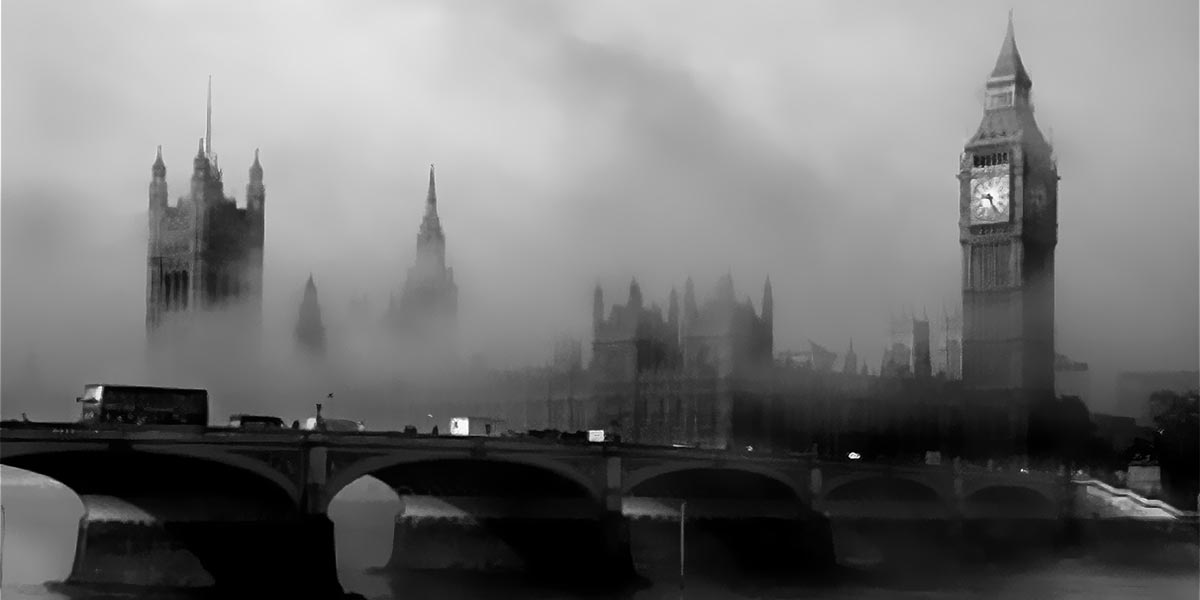
\includegraphics[width=0.8\textwidth]{εικόνες/Marquis-Intelligence-The-Great-Smog-of-London-1952}
      \caption{Η μεγάλη αιθαλομίχλη του Λονδίνου του 1952}
    \label{fig:LondonSmog}
\end{figure}

 Σύμφωνα με επίσημες κυβερνητικές πηγές της εποχής, η αιθαλομίχλη αποτέλεσε τον άμεσο παράγοντα σε 3 χιλιάδες θανάτους μέσα στις 3 πρώτες εβδομάδες εκείνου του Δεκεμβρίου. Όμως, σύμφωνα με μετέπειτα έρευνες, οι θάνατοι που προήρθαν από τις οξείες ή συνεχιζόμενες επιπτώσεις της αιθαλομίχλης στην υγεία των ανθρώπων πρέπει να ήταν στην πραγματικότητα γύρω στις δώδεκα χιλιάδες θανάτους \cite{Bell2001}. Όπως και να έχει, το γεγονός αυτό οδήγησε στην θέσπιση του Clean Air Act 1956 και ήταν σημαντικός καταλύτης στην εξέλιξη της ερευνάς σχετικά με την μόλυνση του ατμοσφαιρικού αέρα \cite{AssociationofDirectorsofPublicHealth2023}.


\begin{figure}[htbp]
  \centering
  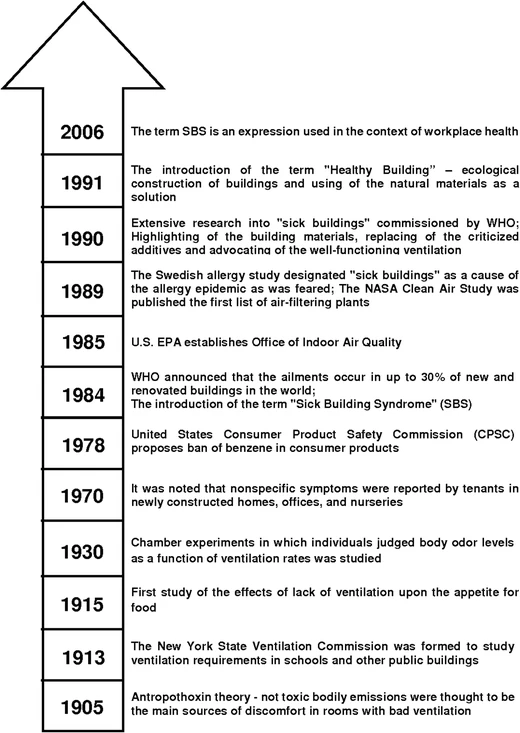
\includegraphics[width=\textwidth]{εικόνες/χρονοδιαγράμμα IAQ.png}
  \caption{Χρονοδιάγραμμα επέκτασης της γνώσης της ποιότητας αέρα.\cite{Śmiełowska2017}}
  \label{fig:χρονοδιαγράμμα IAQ}
\end{figure}

\FloatBarrier % εμποδίζει το float να πάει στο επόμενο section
